% !TeX program = xelatex
% !TeX encoding = UTF-8
% Adapted from billryan/resume (MIT); see TEMPLATE-LICENSE.
% The template definitions are embedded to support the standalone editor.
\documentclass[10pt,a4paper]{article}
\usepackage[top=1.00cm,bottom=1.00cm,left=1.20cm,right=1.20cm,nohead]{geometry}
\usepackage{fontspec}
\usepackage{xeCJK}
\usepackage{graphicx}
\usepackage{enumitem}
\usepackage{titlesec}
\usepackage{fontawesome}
\usepackage[hidelinks]{hyperref}
\usepackage{atbegshi}
\pagestyle{empty}
\setlength{\parindent}{0pt}
\setlength{\parskip}{0pt}
\setlength{\emergencystretch}{2em}
\linespread{1}
\setmainfont{texgyretermes-regular.otf}[BoldFont=texgyretermes-bold.otf,ItalicFont=texgyretermes-italic.otf]
\setsansfont{texgyreheros-regular.otf}[BoldFont=texgyreheros-bold.otf]
\setCJKmainfont[BoldFont=FandolHei-Bold.otf,ItalicFont=FandolKai-Regular.otf]{FandolSong-Regular.otf}
\setCJKsansfont[BoldFont=FandolHei-Bold.otf]{FandolHei-Regular.otf}
% billryan/resume section and dated-subsection layout, tuned for one page.
\titleformat{\section}{\fontsize{12.2}{14}\selectfont\raggedright\bfseries}{}{0em}{}[\titlerule]
\titlespacing*{\section}{0pt}{4pt}{2pt}
\titleformat{\subsection}{\normalsize\raggedright}{}{0em}{}
\titlespacing*{\subsection}{0pt}{3pt}{1pt}
\newcommand{\datedsubsection}[2]{\par\addvspace{3pt}\noindent\makebox[\linewidth][l]{\textbf{#1}\hfill{\fontsize{9}{11}\selectfont #2}}\par\nobreak\vspace{1pt}}
\newcommand{\name}[1]{\centerline{\fontsize{22}{25}\selectfont\bfseries #1}\vspace{5pt}}
\newcommand{\email}[1]{\faEnvelope\ \href{mailto:#1}{#1}}
\newcommand{\phone}[1]{\faPhone\ #1}
\newcommand{\basicInfo}[1]{\centerline{\sffamily\fontsize{9.5}{12}\selectfont #1}}
\newcommand{\tech}[1]{{\fontsize{8.5}{10.5}\selectfont\itshape #1\par}\vspace{1pt}}
\setlist[itemize]{label=\textbullet,leftmargin=1.25em,labelsep=0.45em,
  itemsep=0.7pt,topsep=1pt,parsep=0pt,partopsep=0pt}
\newcount\cvpages
\AtBeginShipout{\global\advance\cvpages by 1
  \ifnum\cvpages>1\PackageError{cv}{Resume exceeds one page}{Shorten the content or adjust spacing.}\fi}
\begin{document}
\fontsize{9.2}{11.2}\selectfont
% Symmetric side columns keep the contact block centered independently of the photo.
\noindent\begin{minipage}[c]{0.14\textwidth}
  \rule{0pt}{1.9cm}
\end{minipage}%
\begin{minipage}[c]{0.72\textwidth}
  \name{李昕潼}
  \basicInfo{\phone{18543740228}\quad\textperiodcentered\quad\email{xintong.li@u.nus.edu}}
\end{minipage}%
\begin{minipage}[c]{0.14\textwidth}
  \raggedleft
  \IfFileExists{assets/resume_photo.png}{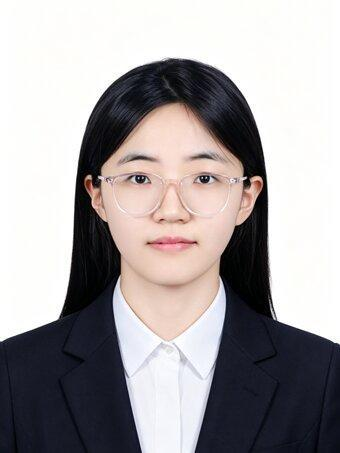
\includegraphics[width=1.5cm]{assets/resume_photo.png}}{\rule{0pt}{1.9cm}}
\end{minipage}\par
\section{\faGraduationCap 教育背景}
\datedsubsection{新加坡国立大学　计算机硕士（MComp）}{2026/08--至今}
\datedsubsection{北京邮电大学　通信工程本科}{2022/09--2026/06}
本科期间均分90.47，专业排名前5\%；获国家奖学金，获评北京市优秀毕业生。\par
\section{\faUsers 实习经历}
\datedsubsection{快手　AI Agent开发工程师（Code Agent）}{2026/05--2026/07}
\tech{LangGraph / OpenCode / Context Engineering / Style Memory / Test-Time Scaling}
参与面向设计稿到可交互应用的Code Agent研发，围绕结构化上下文、分层任务规划、设计风格记忆与推理时迭代优化，改进多页面代码生成流程与效果。\par
\begin{itemize}
\item \textbf{上下文工程：}针对Figma节点逐层展开与多页面长上下文下生成效果不佳的问题，将布局、组件、样式及设计资源组织为页面级结构化表示，结合任务工作区按需加载，优化模型的设计理解与生成上下文。
\item \textbf{分层任务规划：}基于LangGraph将复杂任务拆解为单页面实现、跨页面联动与交互动效补全等阶段，持久化页面上下文与生成产物，支持阶段间信息复用及多页面任务的连续推进。
\item \textbf{面向自进化的风格记忆：}保存并复用设计师的设计风格信息，将历史偏好作为后续任务的生成条件，与当前设计上下文共同指导代码生成，支持跨任务偏好积累与个性化风格一致性。
\item \textbf{推理时优化：}基于OpenCode串联代码生成、执行反馈与多轮修复，利用运行报错指导后续代码修正；分析尺寸异常、字体缺失和布局偏差等失败案例，迭代上下文组织与生成策略。
\end{itemize}
\section{\faCode 项目经历}
\datedsubsection{基于Agent TARS的网页交互质量评测}{2026/03--2026/05}
\tech{Python / Agent TARS / Playwright / VLM / Flask / GUI Automation}
面向大模型生成网页的功能正确性与视觉质量，构建无需参考实现的自动评测流程，覆盖11个领域、54类场景与1,000条需求。\par
\begin{itemize}
\item \textbf{自主交互评测：}基于Agent TARS串联视觉观察、任务规划与浏览器操作，围绕用户需求自主探索页面功能，形成静态感知、Agent交互与动态评分的三阶段评测流程。
\item \textbf{多模态证据与缺陷归因：}融合连续录屏、逐步截图、音频及运行日志，在完整证据采集后统一评分，识别静态截图难以发现的状态更新、交互逻辑与动态效果缺陷，输出功能与美观双维评价。
\item \textbf{项目结果：}完成13个大模型在React与HTML两种生成模式下的评测；在132条需求、528个人工标注实例上，总体成对偏好一致率达61.6\%，较无视频与逐步即时评分方案分别提升4.9和21.0个百分点。
\end{itemize}

\datedsubsection{MiniOneRec：生成式推荐系统}{2026/08--2026/10}
\tech{Python / Sentence-BERT / RQ-VAE / Qwen2.5 / SFT / GRPO / DeepSpeed ZeRO-2}
面向传统推荐系统依赖ID嵌入、难以迁移语义知识的问题，构建端到端生成式推荐框架，将商品语义压缩为离散语义ID，通过大语言模型完成序列生成与偏好对齐。\par
\begin{itemize}
\item \textbf{语义ID构建与约束解码：}使用Sentence-BERT联合编码商品标题与描述，经三层RQ-VAE残差量化生成层次化语义ID（SID）；针对量化碰撞进行迭代去重，并结合约束解码限定合法商品空间，生成SID合法率达100\%。
\item \textbf{多任务监督微调（SFT）：}基于Qwen2.5将用户历史交互转为SID序列，联合语言建模与SID对齐目标开展next-token预测；使用DeepSpeed ZeRO-2在8×A100上完成分布式训练，降低显存占用并加速收敛。
\item \textbf{推荐导向的强化学习（GRPO）：}设计融合命中正确性与排序感知的复合奖励，对SFT模型进行GRPO策略优化；推理阶段结合约束束搜索（Constrained Beam Search），输出合法且去重的推荐候选。
\item \textbf{实验结果：}在Amazon Industrial \& Scientific数据集上，相较传统ID推荐模型，Recall@10提升15.2\%，NDCG@10提升12.8\%。
\end{itemize}
\datedsubsection{基于大模型智能体的网络故障根因定位系统}{2025/12--2026/03}
\tech{Python / Qwen2.5-7B-Instruct / PEFT / LoRA / GRPO / LangChain / ReAct / RAG}
面向网络运维故障定位，结合结构化指标、知识检索与多步推理，实现从观测信息到候选根因的自动化诊断。\par
\begin{itemize}
\item \textbf{设计两阶段蒸馏式SFT数据流程：}基于TeleLogs，围绕工程参数、用户观测指标、症状描述与候选根因构建2,400条样本；先以排除、矛盾、规则、统计四类专家策略生成推理轨迹，再由教师模型整合、压缩与标准化正确轨迹，形成高质量RCA训练数据。
\item \textbf{开展参数高效训练与策略优化：}使用PEFT/LoRA对Qwen2.5-7B-Instruct进行监督微调，进一步结合GRPO优化最终根因判别，提升复杂故障场景下的输出稳定性与决策准确率。
\item \textbf{构建ReAct诊断智能体：}基于LangChain封装表格解析、故障区间识别、服务小区几何及邻区干扰分析工具，将原始数据转为结构化诊断证据；结合规则知识库与RAG开展多步推理，增强诊断的可解释性。
\item \textbf{实验结果：}Pass@1由基础模型的12.04\%提升至微调后的53.59\%，引入Agent后达到76.50\%；Pass@4对应由12.50\%提升至54.86\%和78.36\%。
\end{itemize}
\section{\faCogs 技能特长}
\textbf{开发环境：}Linux、Shell、Git、Conda、远程GPU服务器。\par
\textbf{模型训练：}LoRA/QLoRA、PEFT、GRPO；数据构建、领域微调与效果评测。\par
\textbf{智能体开发：}LangGraph、LangChain、ReAct、Tool Calling、Multi-Agent。\par
\end{document}
